%	This LaTeX file is written by Zhiyang Ong as a template for creating presentation slides.

%	The MIT License (MIT)

%	Copyright (c) <2014> <Zhiyang Ong>

%	Permission is hereby granted, free of charge, to any person obtaining a copy of this software and associated documentation files (the "Software"), to deal in the Software without restriction, including without limitation the rights to use, copy, modify, merge, publish, distribute, sublicense, and/or sell copies of the Software, and to permit persons to whom the Software is furnished to do so, subject to the following conditions:

%	The above copyright notice and this permission notice shall be included in all copies or substantial portions of the Software.

%	THE SOFTWARE IS PROVIDED "AS IS", WITHOUT WARRANTY OF ANY KIND, EXPRESS OR IMPLIED, INCLUDING BUT NOT LIMITED TO THE WARRANTIES OF MERCHANTABILITY, FITNESS FOR A PARTICULAR PURPOSE AND NONINFRINGEMENT. IN NO EVENT SHALL THE AUTHORS OR COPYRIGHT HOLDERS BE LIABLE FOR ANY CLAIM, DAMAGES OR OTHER LIABILITY, WHETHER IN AN ACTION OF CONTRACT, TORT OR OTHERWISE, ARISING FROM, OUT OF OR IN CONNECTION WITH THE SOFTWARE OR THE USE OR OTHER DEALINGS IN THE SOFTWARE.

%	Email address: echo "cukj -wb- 23wU4X5M589 TROJANS cqkH wiuz2y 0f Mw Stanford" | awk '{ sub("23wU4X5M589","F.d_c_b. ") sub("Stanford","d0mA1n"); print $5, $2, $8; print " "; for (i=1; i<=1; i++) print "6\b"; print $9, $7, $6 }' | sed y/kqcbuHwM62z/gnotrzadqmC/ | tr 'q' ' ' | tr -d "\n" | tr -d 'ir' | tr y "\n"



%%%%%%%%%%%%%%%%%%%%%%%%%%%%%%%%%%%%%%%%%%%%%%
%	Preamble

%	Use the Beamer package to create the presentation slides.
\documentclass[xcolor={usenames,dvipsnames},hyperref={hyperindex,bookmarks}]{beamer}
%	Background color: Set it to blue.
%\setbeamercolor{background canvas}{bg=blue}
%	\setbeamercolor{normal text}{bg=white,fg=yellow}
%\setbeamercolor{normal text}{fg=white}
%	\setbeamercolor{title}{fg=yellow,bg=white}
%\setbeamercolor{title}{fg=yellow}
%	\setbeamercolor{titlelike}{fg=yellow,bg=white}
%\setbeamercolor{block title alerted}{fg=white,bg=yellow}



%%%%%%%%%%%%%%%%%%%%%%%%%%%%%%%%%%%%%%%%%%%%%%
%	Information indicating Copyright information for Creative Commons license.
\usepackage{ccicons}
\usepackage{cclicenses}
\usepackage[
    type={CC},
    modifier={by-nc-nd},
    version={4.0},
]{doclicense}




%%%%%%%%%%%%%%%%%%%%%%%%%%%%%%%%%%%%%%%%%%%%%%
%	Table of Contents
\AtBeginSection[]
{
	\begin{frame}
%		\frametitle{\textcolor{yellow}{Table of Contents}}
		\frametitle{Table of Contents}
%		\textcolor{yellow}{\tableofcontents[currentsection]}
		\tableofcontents[currentsection,currentsubsection]
	\end{frame}
}

%	IMPORTANT: Note that entries for the Table of Contents are indicated by sections and subsections.


%%%%%%%%%%%%%%%%%%%%%%%%%%%%%%%%%%%%%%%%%%%%%%
%	Main document
\begin{document}


%%%%%%%%%%%%%%%%%%%%%%%%%%%%%%%%%%%%%%%%%%%%%%
%	Slide 1

%	Set the background picture.
{
\usebackgroundtemplate{
\includegraphics[width=\paperwidth,height=\paperheight,keepaspectratio]{./pics/backgnd}}

	\title[Cover Title]
	{Title of My Presentation}
	\subtitle{A Presentation Made In \LaTeX}
	\author{Nome1 Cognome1\inst{1} \and Nome2 Cognome2\inst{2}}
	\institute{
		\inst{1}
		Department1, Division1 \\
		Organization1 \\
		City1, State1 \\
		Country1
		\and
		\inst{2}
		Department2, Division2 \\
		Organization2 \\
		City2, State2 \\
		Country2
	}
	\date{\today}	% (optional)
	\subject{Subject Title}
	\frame{\titlepage}
%	For setting the background picture.
}


%%%%%%%%%%%%%%%%%%%%%%%%%%%%%%%%%%%%%%%%%%%%%
%
%	Copyright Information


\begin{frame}
	\begin{center} 
	Copyright \copyright\ \the\year{} by Zhiyang Ong
	\end{center}
	\doclicenseThis
\end{frame}

%%%%%%%%%%%%%%%%%%%%%%%%%%%%%%%%%%%%%%%%%%%%%%
%	Section One
\section{Section One}

%%%%%%%%%%%%%%%%%%%%%%%%%%%%%%%%%%%%%%%%%%%%%%
%	Acknowledgments
%	Slide 3

\begin{frame}
	\frametitle{Acknowledgments}
	Name1, Organization1 \\
	\ \\
	Name2, Organization2 \\
	\ \\
	Name3, Organization3
\end{frame}

%%%%%%%%%%%%%%%%%%%%%%%%%%%%%%%%%%%%%%%%%%%%%%
%	Section Two
\section{Section Two}


%%%%%%%%%%%%%%%%%%%%%%%%%%%%%%%%%%%%%%%%%%%%%%
%	Subsection 2.1
\subsection{Subsection 2.1}


%%%%%%%%%%%%%%%%%%%%%%%%%%%%%%%%%%%%%%%%%%%%%%
%	Slide 4
\begin{frame}
	\frametitle{Slide Title 4}
	\framesubtitle{Slide Subtitle 4}
	
	\begin{columns}[t]			% Contents are top vertically aligned
		\begin{column}[T]{5cm}	% Each column can also be its own environment
		
		Statement 1. \\
		\ \\
		Statement 2. \\
		\ \\
		Statement 3.
		\end{column}
		
		\begin{column}[T]{5cm}	% Alternative top-align that's better for graphics
			\begin{figure}
			\centering
			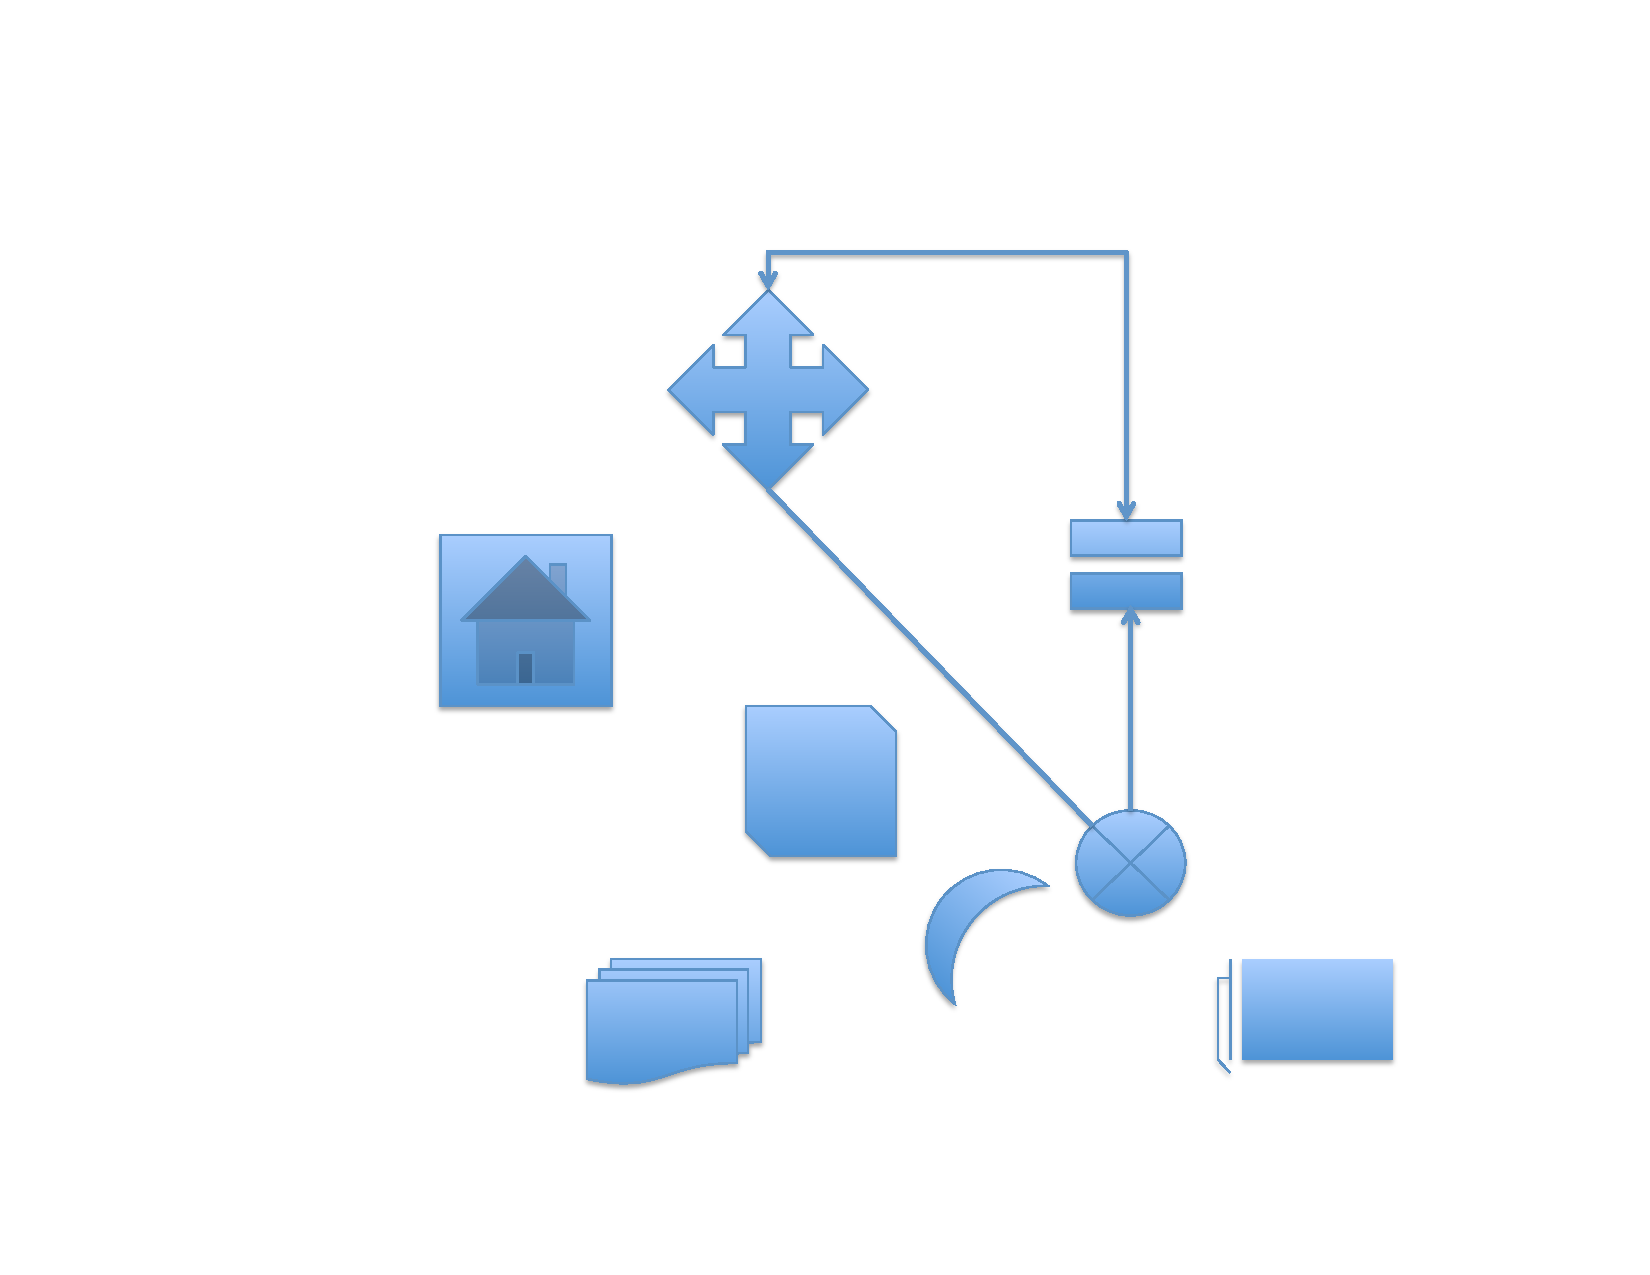
\includegraphics[height=2in]{./pics/my_figure}
			\caption{My caption \cite{Petroski1992,Kopka2004}}
			\end{figure}
		\end{column}
	\end{columns}
\end{frame}

%%%%%%%%%%%%%%%%%%%%%%%%%%%%%%%%%%%%%%%%%%%%%%
%	Subsection 2.2
\subsection{Subsection 2.2}

%%%%%%%%%%%%%%%%%%%%%%%%%%%%%%%%%%%%%%%%%%%%%%
%	Slide 5
\begin{frame}
	\frametitle{Slide Title 5}
	\framesubtitle{Slide Subtitle 5.}
	
	Statement 1 \cite{vanDongen2012}. \\
	\ \\
	Statement 2. \\
	\ \\
	Statement 3.
\end{frame}

%%%%%%%%%%%%%%%%%%%%%%%%%%%%%%%%%%%%%%%%%%%%%%
%	Section 3
\section{Section 3}

%%%%%%%%%%%%%%%%%%%%%%%%%%%%%%%%%%%%%%%%%%%%%%
%	Slide 6
\begin{frame}
	\frametitle{Slide Title 6}
	\framesubtitle{Slide Subtitle 6.}
	
	\begin{figure}
		\centering
		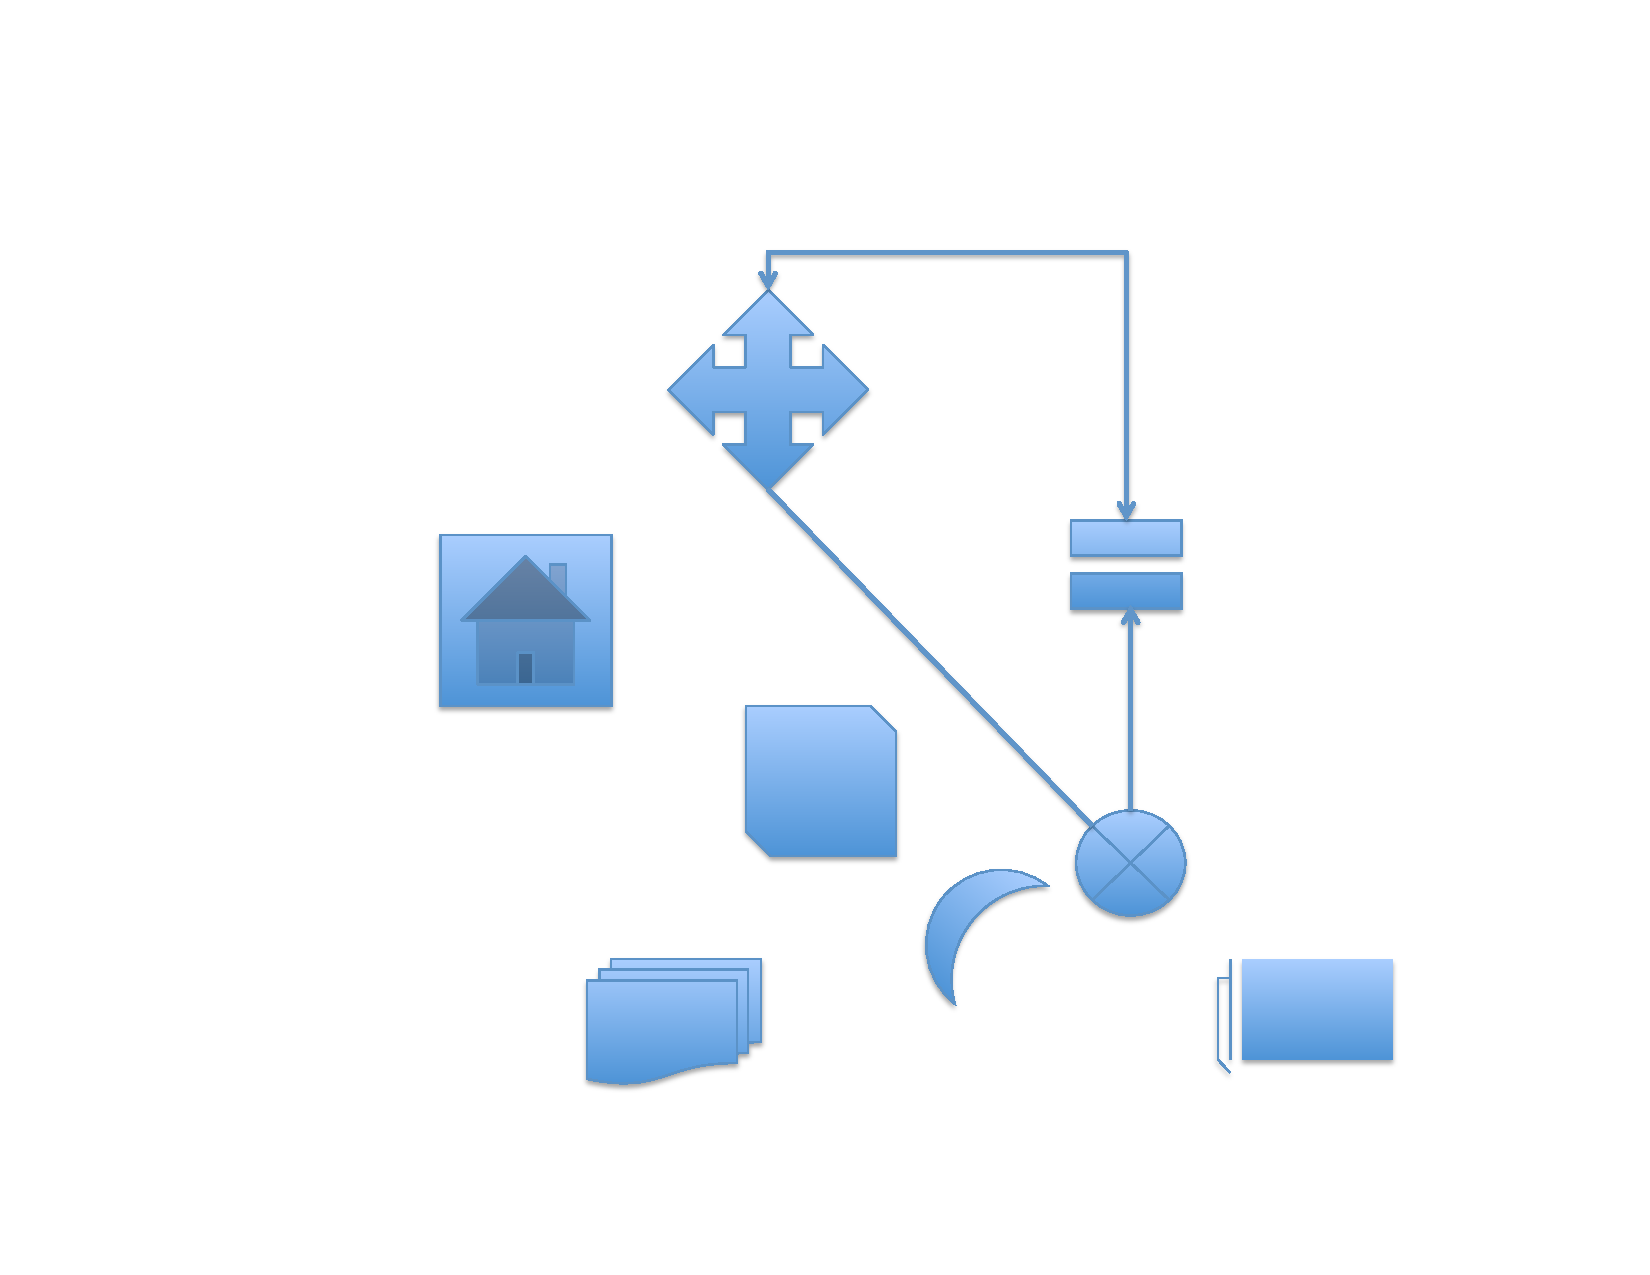
\includegraphics[height=2.6in]{./pics/my_figure}
		\caption{Caption \#2}
	\end{figure}
\end{frame}




%%%%%%%%%%%%%%%%%%%%%%%%%%%%%%%%%%%%%%%%%%%%%
%	Slide 7
%	References
{\linespread{1}
\begin{frame}
	\frametitle{References}
	\bibliographystyle{plain}
	\bibliography{references/references}
\end{frame}
}
%%%%%%%%%%%%%%%%%%%%%%%%%%%%%%%%%%%%%%%%%%%%%
\end{document}